%%%%%%%%%%%%%%%%%%%%%%%%%%%%%%%%%%%%%%%%%
% Beamer Presentation
% LaTeX Template
% Version 2.0 (March 8, 2022)
%
% This template originates from:
% https://www.LaTeXTemplates.com
%
% Author:
% Vel (vel@latextemplates.com)
%
% License:
% CC BY-NC-SA 4.0 (https://creativecommons.org/licenses/by-nc-sa/4.0/)
%
%%%%%%%%%%%%%%%%%%%%%%%%%%%%%%%%%%%%%%%%%

%----------------------------------------------------------------------------------------
%	PACKAGES AND OTHER DOCUMENT CONFIGURATIONS
%----------------------------------------------------------------------------------------
\documentclass[
  24pt, % Set the default font size, options include: 8pt, 9pt, 10pt, 11pt, 12pt, 14pt, 17pt, 20pt
  %t, % Uncomment to vertically align all slide content to the top of the slide, rather than the default centered
  aspectratio=169, % Uncomment to set the aspect ratio to a 16:9 ratio which matches the aspect ratio of 1080p and 4K screens and projectors
]{beamer}

\graphicspath{{Images/}{./}} % Specifies where to look for included images (trailing slash required)

\usepackage{booktabs} % Allows the use of \toprule, \midrule and \bottomrule for better rules in tables

%----------------------------------------------------------------------------------------
%	SELECT LAYOUT THEME
%----------------------------------------------------------------------------------------

% Beamer comes with a number of default layout themes which change the colors and layouts of slides. Below is a list of all themes available, uncomment each in turn to see what they look like.

%\usetheme{default}
%\usetheme{AnnArbor}
%\usetheme{Antibes}
%\usetheme{Bergen}
%\usetheme{Berkeley}
%\usetheme{Berlin}
\usetheme{Boadilla} %me gusta
%\usetheme{CambridgeUS}
%\usetheme{Copenhagen}
%\usetheme{Darmstadt}
%\usetheme{Dresden}
%\usetheme{Frankfurt}
%\usetheme{Goettingen} %dos dos
%\usetheme{Hannover} %dos dos
%\usetheme{Ilmenau}
%\usetheme{JuanLesPins}
%\usetheme{Luebeck}
%\usetheme{Madrid}
%\usetheme{Malmoe}
%\usetheme{Marburg}
%\usetheme{Montpellier}
%\usetheme{PaloAlto}
%\usetheme{Pittsburgh}
%\usetheme{Rochester} %muy flat
%\usetheme{Singapore}
%\usetheme{Szeged}
%\usetheme{Warsaw}

%----------------------------------------------------------------------------------------
%	SELECT COLOR THEME
%----------------------------------------------------------------------------------------

% Beamer comes with a number of color themes that can be applied to any layout theme to change its colors. Uncomment each of these in turn to see how they change the colors of your selected layout theme.

%\usecolortheme{albatross}
%\usecolortheme{beaver}
%\usecolortheme{beetle}
%\usecolortheme{crane}
%\usecolortheme{dolphin}
%\usecolortheme{dove}
%\usecolortheme{fly}
%\usecolortheme{lily} %default
%\usecolortheme{monarca}
%\usecolortheme{seagull}
%\usecolortheme{seahorse}
%\usecolortheme{spruce}
%\usecolortheme{whale}
%\usecolortheme{wolverine}

%----------------------------------------------------------------------------------------
%	SELECT FONT THEME & FONTS
%----------------------------------------------------------------------------------------

% Beamer comes with several font themes to easily change the fonts used in various parts of the presentation. Review the comments beside each one to decide if you would like to use it. Note that additional options can be specified for several of these font themes, consult the beamer documentation for more information.

\usefonttheme{default} % Typeset using the default sans serif font
%\usefonttheme{serif} % Typeset using the default serif font (make sure a sans font isn't being set as the default font if you use this option!)
%\usefonttheme{structurebold} % Typeset important structure text (titles, headlines, footlines, sidebar, etc) in bold
%\usefonttheme{structureitalicserif} % Typeset important structure text (titles, headlines, footlines, sidebar, etc) in italic serif
%\usefonttheme{structuresmallcapsserif} % Typeset important structure text (titles, headlines, footlines, sidebar, etc) in small caps serif

%------------------------------------------------

%\usepackage{mathptmx} % Use the Times font for serif text
\usepackage{palatino} % Use the Palatino font for serif text

\usepackage[ruled,vlined]{algorithm2e}
%\usepackage{helvet} % Use the Helvetica font for sans serif text
\usepackage[default]{opensans} % Use the Open Sans font for sans serif text
\usepackage[spanish]{babel}
\usepackage{dirtree}
\usepackage{xcolor}
%\usepackage[default]{FiraSans} % Use the Fira Sans font for sans serif text
%\usepackage[default]{lato} % Use the Lato font for sans serif text

\usepackage[scaled]{helvet}
\usepackage[round]{natbib}
%\newcommand{\newblock}{}

\usepackage{rotating}

\newcommand\FourQuad[4]{%
  \begin{minipage}[b][.33\textheight][t] 
    {.48\textwidth}#1\end{minipage}\hfill%
    \begin{minipage}[b][.33\textheight][t] 
      {.48\textwidth}#2\end{minipage}\\[0.5em]
      \begin{minipage}[b][.33\textheight][t] 
        {.48\textwidth}#3\end{minipage}\hfill
        \begin{minipage}[b][.33\textheight][t] 
          {.48\textwidth}#4\end{minipage}%
}

\usepackage{tikz}
%\usetikzlibrary{arrows,shapes,positioning,shadows,trees,quotes}


%\tikzset{
%  basic/.style  = {draw, text width=2cm, drop shadow, font=\sffamily, rectangle},
%  root/.style   = {basic, rounded corners=2pt, thin, align=center,
%                   fill=green!30},
%  level 2/.style = {basic, rounded corners=6pt, thin,align=center, fill=green!60,
%                   text width=8em},
%  level 3/.style = {basic, thin, align=left, fill=pink!60, text width=6.5em}
%}

\usetikzlibrary{calc}

\tikzstyle{part} = [rectangle, rounded corners, minimum width=3cm, minimum height=1cm,     align=center, draw=black]
\tikzstyle{chapter} = [rectangle, rounded corners, minimum width=3cm, minimum height=1cm,     align=center, draw=black, text width=3.5cm]
\tikzstyle{arrow} = [thick, ->]

\usepackage{array} % needed for \arraybackslash
\usepackage{graphicx}
\usepackage{adjustbox} % for \adjincludegraphics

\usepackage{subcaption}
\usepackage{bibentry}
%\bibliographystyle{apalike}
\usepackage{chngcntr}
\usepackage{lipsum}% http://ctan.org/pkg/lipsum
\usepackage{hanging}% http://ctan.org/pkg/hanging

\usepackage{xcolor,colortbl}
\usepackage{multirow}

\usepackage{animate}
\usepackage{multicol}
\usepackage{tabularx,booktabs}
\usepackage{forloop}
\usepackage{ragged2e}

\usepackage{bbding} %palomitas checkmark
\usepackage{pifont}
\usepackage{lipsum,tabularx}

\newcounter{loopcntr}

%----------------------------------------------------------------------------------------
%	SELECT INNER THEME
%----------------------------------------------------------------------------------------

% Inner themes change the styling of internal slide elements, for example: bullet points, blocks, bibliography entries, title pages, theorems, etc. Uncomment each theme in turn to see what changes it makes to your presentation.

\useinnertheme{circles}

%----------------------------------------------------------------------------------------
%	SELECT OUTER THEME
%----------------------------------------------------------------------------------------

% Outer themes change the overall layout of slides, such as: header and footer lines, sidebars and slide titles. Uncomment each theme in turn to see what changes it makes to your presentation.

\setbeamertemplate{footline}[frame number] % Uncomment this line to replace the footer line in all slides with a simple slide count
\setbeamertemplate{navigation symbols}{} % Uncomment this line to remove the navigation symbols from the bottom of all slides

%----------------------------------------------------------------------------------------
%	PRESENTATION INFORMATION
%----------------------------------------------------------------------------------------

\title[PRESENTACION 3]{%\centering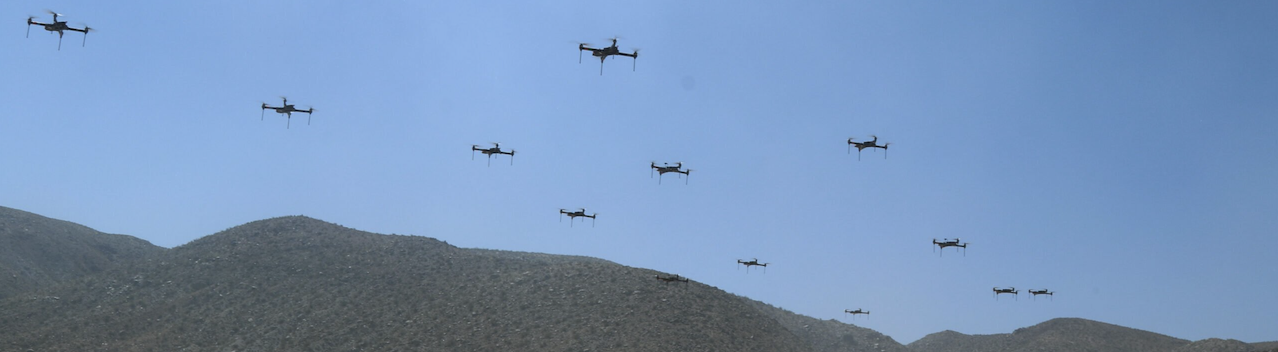
\includegraphics[width=10cm]{swarm_drones}\\
  Estrategias para la exploración coordinada multi-VANT} % The short title in the optional parameter appears at the bottom of every slide, the full title in the main parameter is only on the title page

%\subtitle{Optional Subtitle} % Presentation subtitle, remove this command if a subtitle isn't required

\author[]{Luis Alberto Ballado Aradias\\[\baselineskip]
  \small{{Asesores:} \\
    \and\\Dr. José Gabriel Ramírez-Torres
    \and\\Dr. Eduardo Rodriguez-Tello }}

\institute[CINVESTAV]{
  CINVESTAV UNIDAD TAMAULIPAS \\
  %\smallskip \textit{luis.ballado@cinvestav.mx}
} % Your institution, the optional parameter can be used for the institution shorthand and will appear on the bottom of every slide after author names, while the required parameter is used on the title slide and can include your email address or additional information on separate lines


\date[\today]{Cd. Victoria, Tamaulipas - 13 Marzo 2024} % Presentation date or conference/meeting name, the optional parameter can contain a shortened version to appear on the bottom of every slide, while the required parameter value is output to the title slide

%\titlegraphic{\hspace*{8.75cm}~%
%   
\includegraphics[width=0.8cm]{cinvestavlogo}
%}

%----------------------------------------------------------------------------------------

\counterwithin*{footnote}{page}
\newcommand\footcite[1]{\footnote{\bibentry{#1}}\label{\thepage:#1}}
\newcommand\secondcite[1]{\textsuperscript{\ref{\thepage:#1}}}

\newcommand{\rpt}[2][1]{%
  \forloop{loopcntr}{0}{\value{loopcntr}<#1}{#2}%
}
\newcommand{\on}[1][1]{
  \forloop{loopcntr}{0}{\value{loopcntr}<#1}{&\cellcolor{gray}}
}
\newcommand{\onok}[1][1]{
  \forloop{loopcntr}{0}{\value{loopcntr}<#1}{&\cellcolor{green}}
}
\newcommand{\off}[1][1]{
  \forloop{loopcntr}{0}{\value{loopcntr}<#1}{&\cellcolor{white}}
}

\addtolength{\textheight}{90pt}

\newcommand{\I}{\mathbb{I}}
\newcommand{\K}{\mathbb{K}}
\newcommand{\N}{\mathbb{N}}
\newcommand{\Q}{\mathbb{Q}}
\newcommand{\R}{\mathbb{R}}
\newcommand{\Z}{\mathbb{Z}}

\newcommand{\specialcell}[2][c]{%
  \begin{tabular}[#1]{@{}c@{}}#2\end{tabular}}


\begin{document}

%----------------------------------------------------------------------------------------
%	TITLE SLIDE
%----------------------------------------------------------------------------------------

\begin{frame}
  \titlepage % Output the title slide, automatically created using the text entered in the PRESENTATION INFORMATION block above
\end{frame}

%----------------------------------------------------------------------------------------
%	TABLE OF CONTENTS SLIDE
%----------------------------------------------------------------------------------------

% The table of contents outputs the sections and subsections that appear in your presentation, specified with the standard \section and \subsection commands. You may either display all sections and subsections on one slide with \tableofcontents, or display each section at a time on subsequent slides with \tableofcontents[pausesections]. The latter is useful if you want to step through each section and mention what you will discuss.
\AtBeginSection[]
{
  \begin{frame}
    \frametitle{Contenido} % Slide title, remove this command for no title
    \tableofcontents[currentsection] % Output the table of contents (all sections on one slide)
    %\tableofcontents[pausesections] % Output the table of contents (break sections up across separate slides)
  \end{frame}
}

\pretocmd{\tableofcontents}{\thispagestyle{empty}}{}{}

%----------------------------------------------------------------------------------------
%	PRESENTATION BODY SLIDES
%----------------------------------------------------------------------------------------

\section{Resumen}
\begin{frame}{Resumen}
  \bigskip % Vertical whitespace
  \centering
  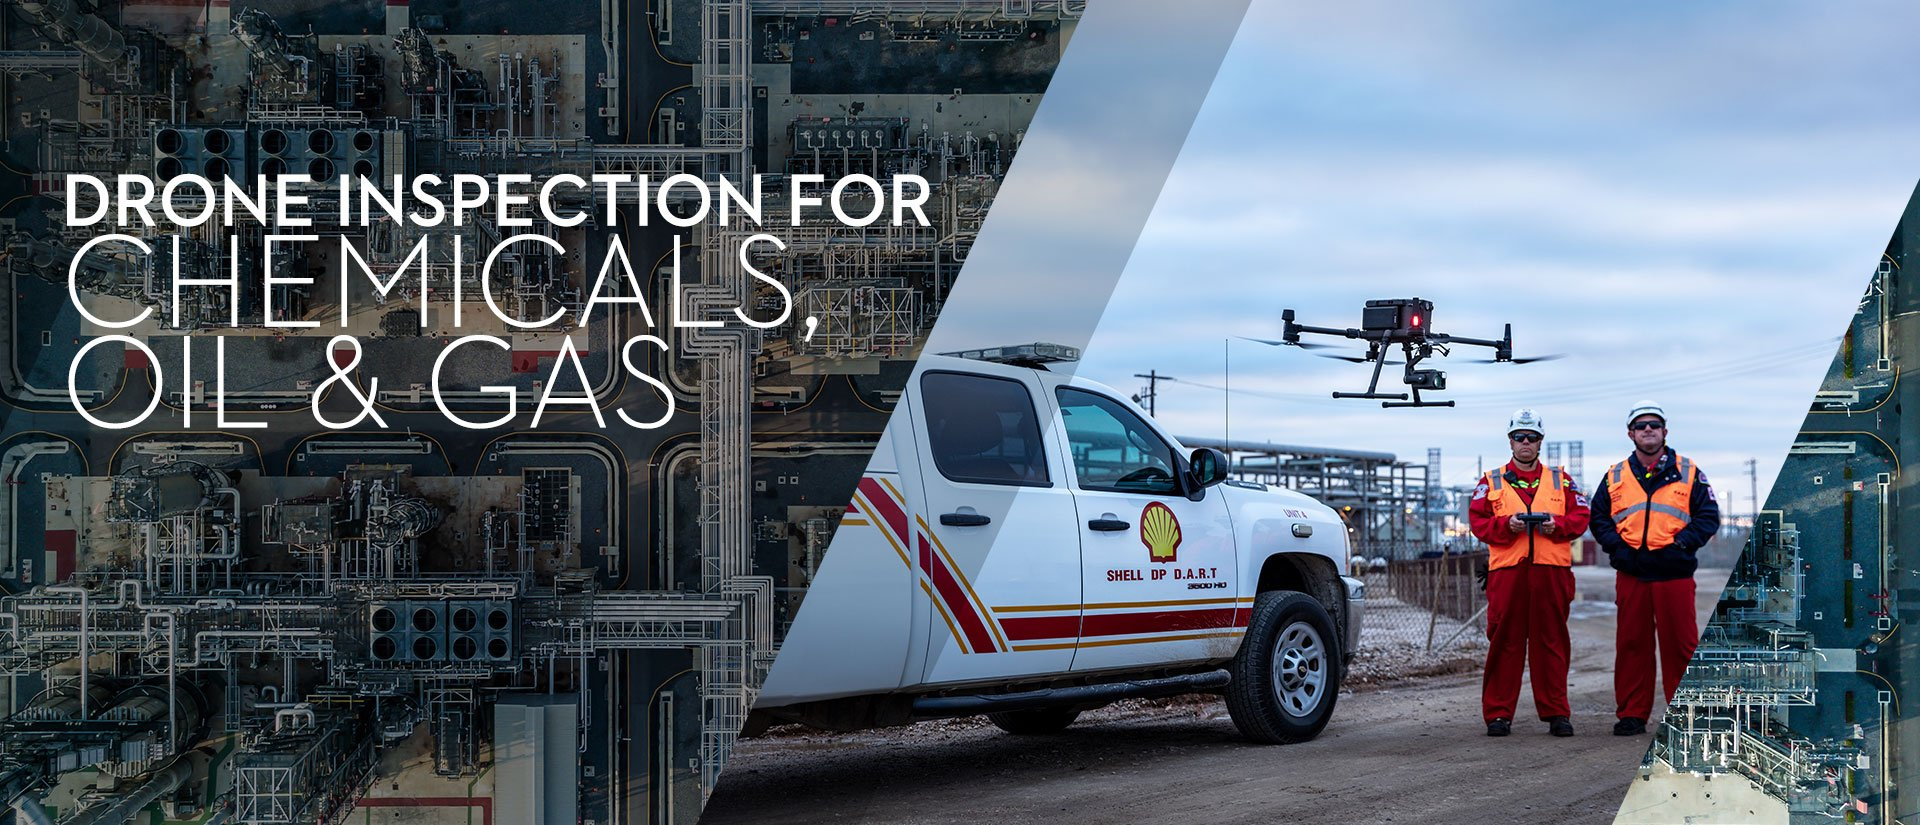
\includegraphics[width=0.45\textwidth,height=0.35\textheight]{DJI_B4}
  \hfil
  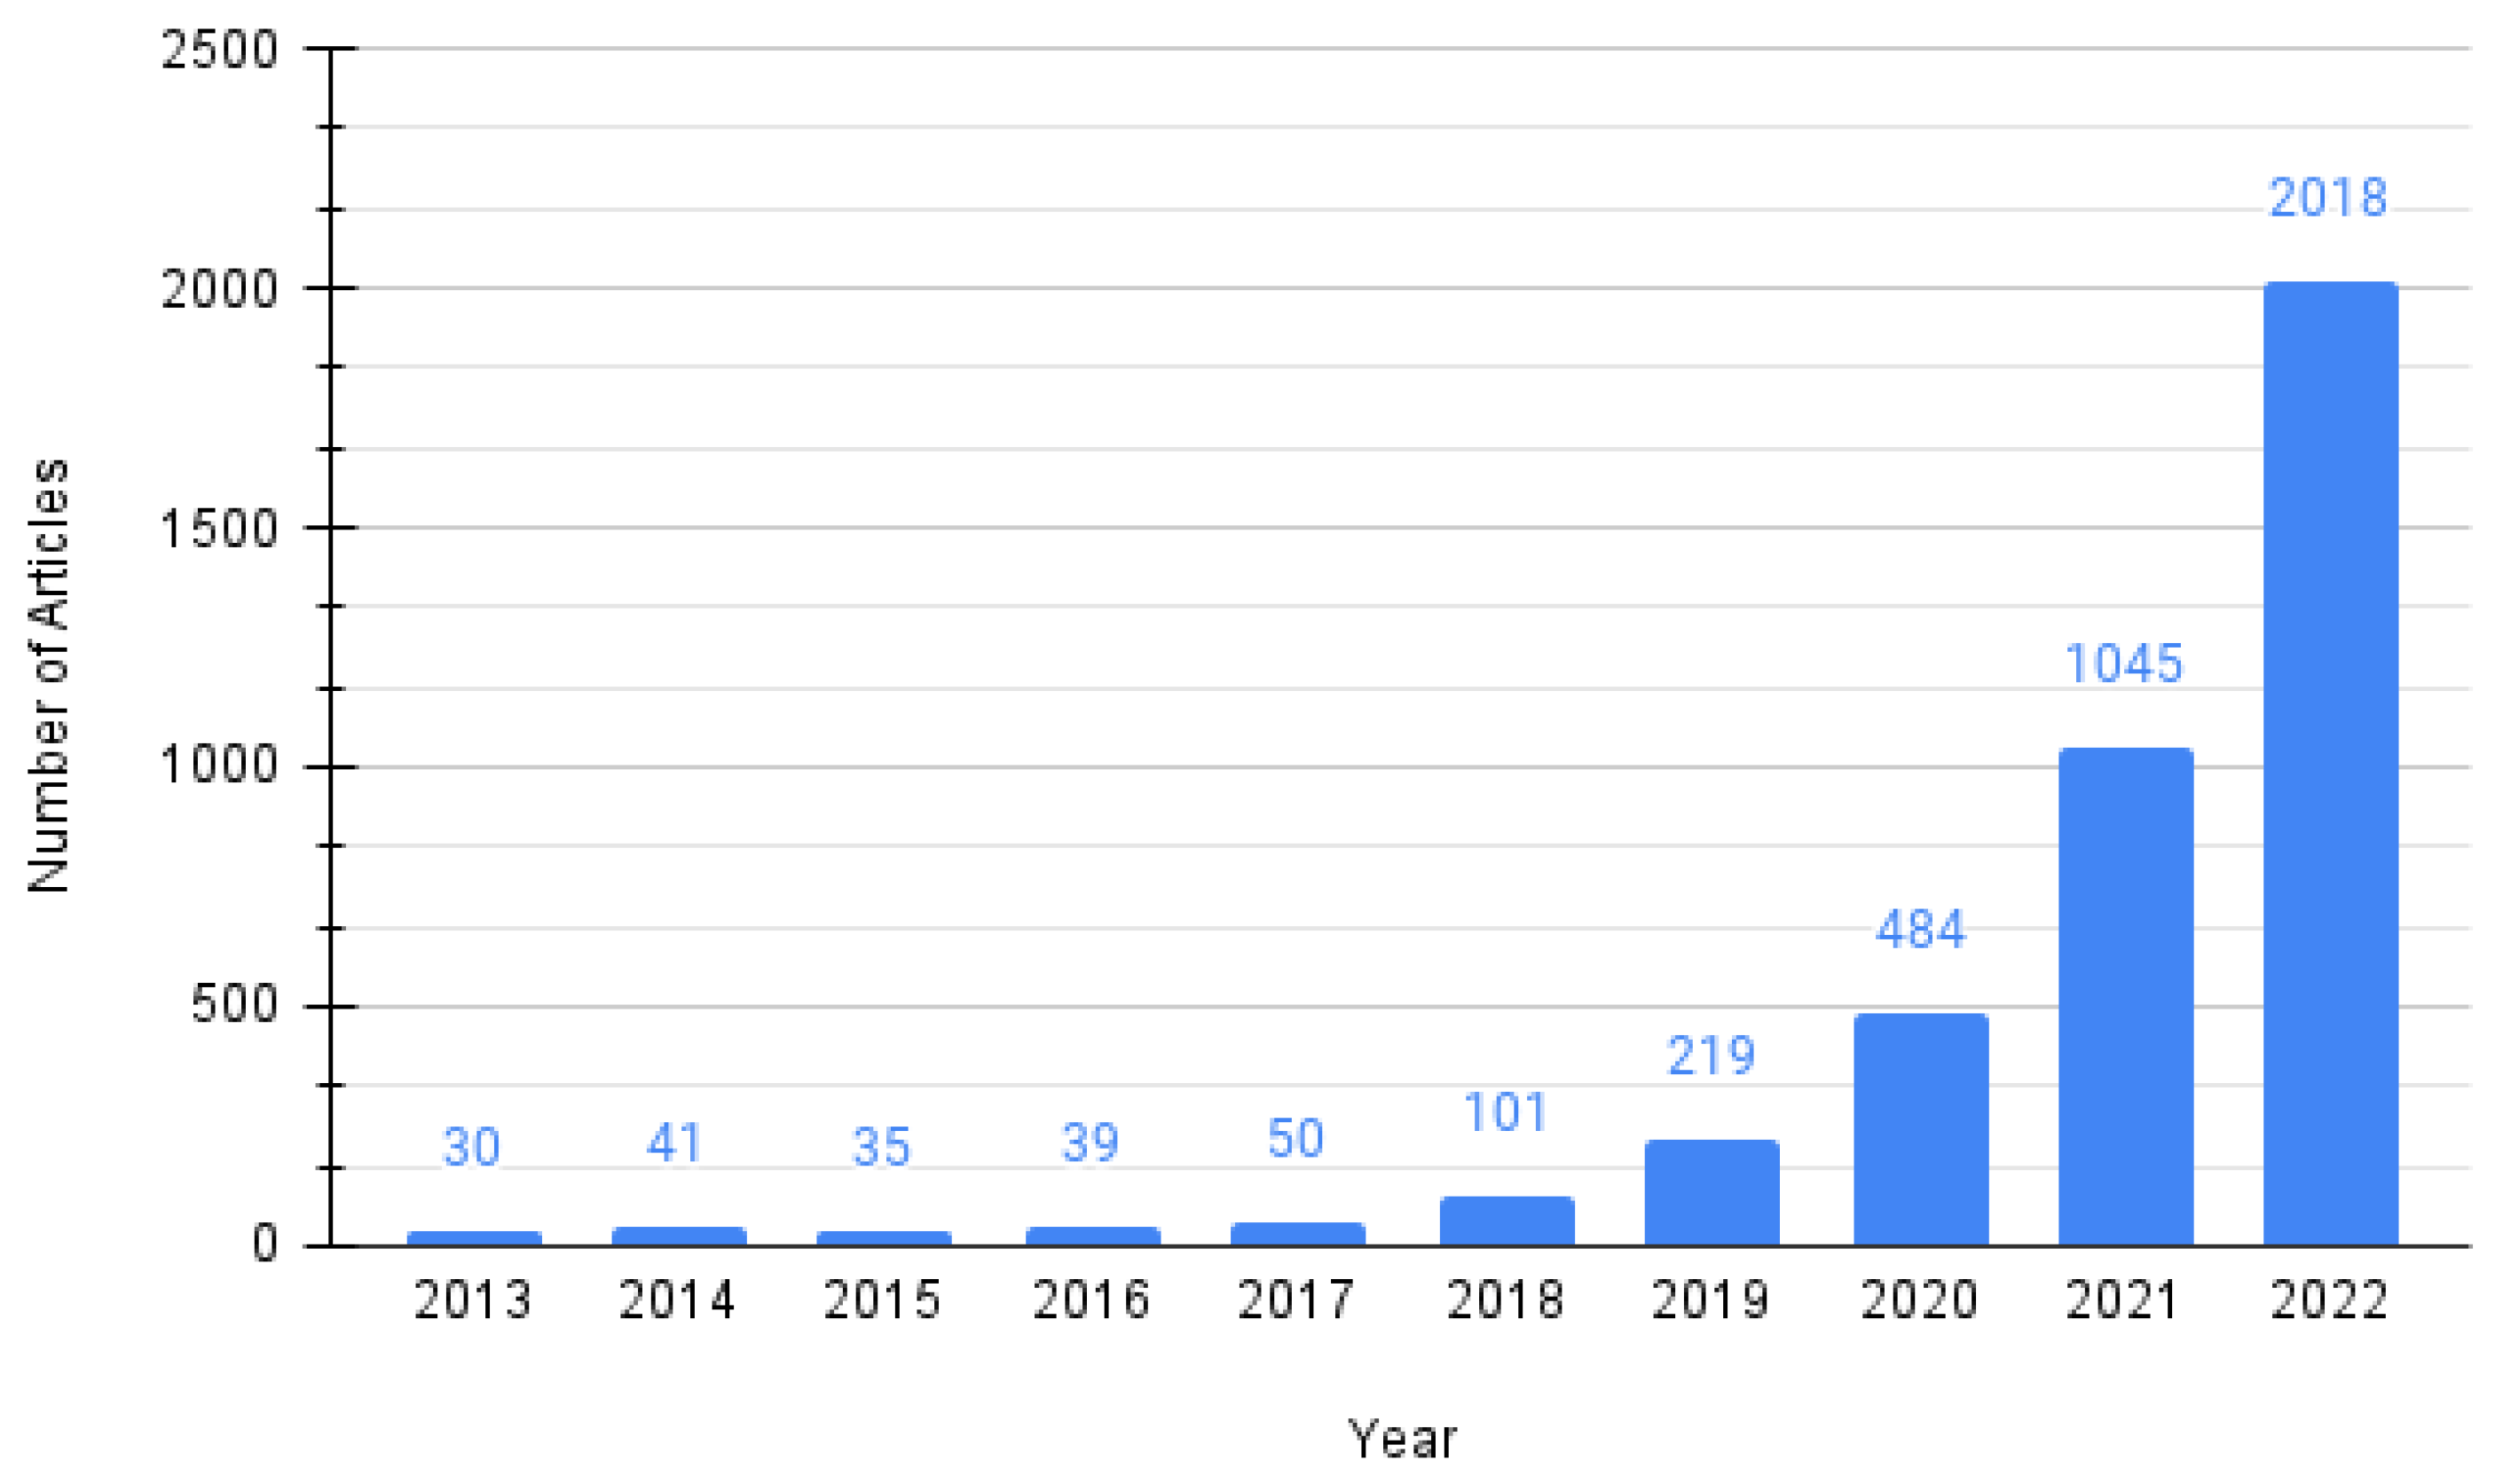
\includegraphics[width=0.45\textwidth,height=0.35\textheight]{drones-07-00236-g001.png}\footnotemark
  \vspace{2pt}\\
  
  \begin{itemize}
  \item \textbf{Aplicaciones} en lugares inaccesibles o peligrosos.
  \item \textbf{Múltiples VANT} pueden reducir el tiempo de exploración y aumentar la confianza del sistema.
  \item \textbf{Limitaciones} en carga, procesamiento y batería influyen en el tiempo de vuelo.
  \item \textbf{UAV} {\tiny(Vehículo Aéreo No Tripulado VANT)}  $\implies$ \textbf{UAS} {\tiny(Sistemas Aéreos No Tripulado SANT)}
  \end{itemize}
  
  \footnotetext{UAV in the advent of the twenties: Where we stand and what is next [\cite{Nex2022}]}
  %
\includegraphics[width=0.45\textwidth,height=0.35\textheight]{DJI_B5}$^\dag$ 
  %\hfil
  %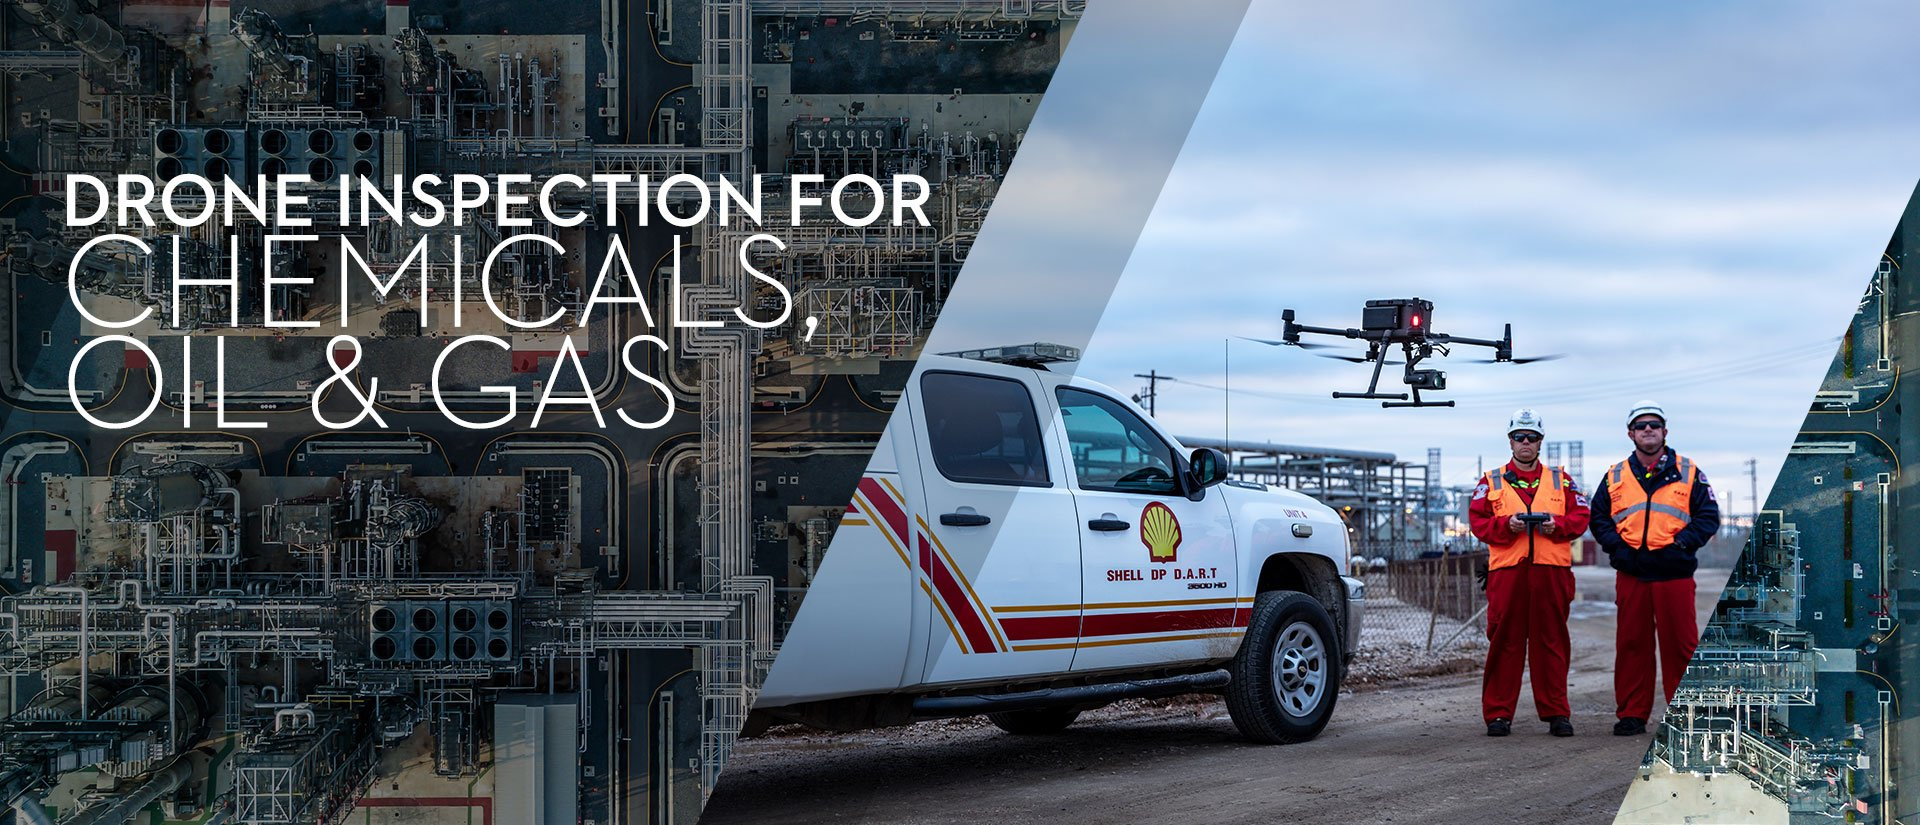
\includegraphics[width=0.45\textwidth,height=0.35\textheight]{DJI_B4}$^\dag$\\
  %\rule{0in}{1.2em}$^\dag$ \small Inspecciones con VANT basadas en los mejores casos de uso\\
  %\tiny \url{https://enterprise-insights.dji.com/blog/complete-guide-to-drone-inspections}
\end{frame}

\section{Sistema Multi-agente}
\begin{frame}{Sistema Multi-agente}

  %Un sistema multi-agente, es un sistema que consta de multiples entidades autonomas, llamadas agentes, que estan situados en el medio ambiente por lo que los agentes pueden estar parcialmente observados y en el ambiente pueden actuar y cooperar para completar el objetivo del sistema.
  \bigskip % Vertical whitespace
  \centering
  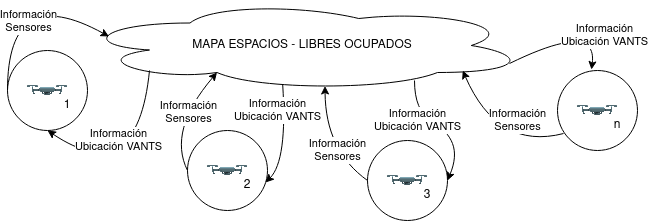
\includegraphics[width=12cm]{problema}\\
\end{frame}

\subsection{VANTS Autónomos}
\begin{frame}{Exploración}
  %\textbf{Exploración}\\
  \bigskip % Vertical whitespace
  %Exploración es una tarea fundamental en robots autónomos.
  El objetivo es crear un mapa de un ambiente desconocido.\\
  \bigskip % Vertical whitespace
  \centering
  
\includegraphics[width=7cm]{exploracion}\\
  
  \begin{itemize}
  \item \textbf{Sensar}
  \item \textbf{Creación Mapa} 
  \item \textbf{Localización en Mapa}
  \item \textbf{Exploración} Aumentar la base de conocimiento del Mapa
  \item \textbf{Planificación trayectoria} Trayectorias hacia nuevas fronteras 
  \item \textbf{Control} Toma de decisiones y ejecución de trayectorias 
  \end{itemize}

  \alert{- El ciclo se repite hasta completar la exploración -}
  
\end{frame}

\begin{frame}
  
  \begin{itemize}
  \item Conjunto de Agentes (VANTS) $V = \{V_1,V_2,V_3,...,V_n\}$
    \bigskip % Vertical whitespace
    \begin{itemize}
    \item Comandos control $u(t) = \{u_1,u_2,u_3,...,u_n\}$
     \item Mediciones $Z(t) = \{z_1,z_2,z_3,...,z_n\}$
     \item Trayectoria  $X(t) = \{x_1,x_2,x_3,...,x_n\}$
     \item Lista de fronteras $F = \{f_1,f_2,f_3,...,f_n\}$
     \item Mapa $m$
    \end{itemize}
  \end{itemize}

  \bigskip % Vertical whitespace

  \center{Asignar fronteras a cada VANT para reducir el tiempo total de exploración}
  
\end{frame}

\begin{frame}
  \textbf{Arquitectura}
  \begin{figure}
    \centering
    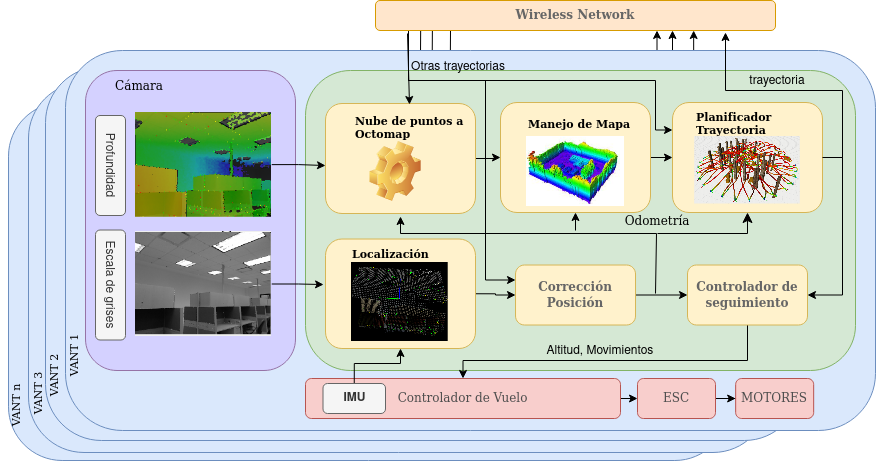
\includegraphics[width=15cm]{arquitectura}
  \end{figure}
\end{frame}

\subsubsection{Control VANT}
\begin{frame}{Control VANT}
  \begin{figure}
    \centering
    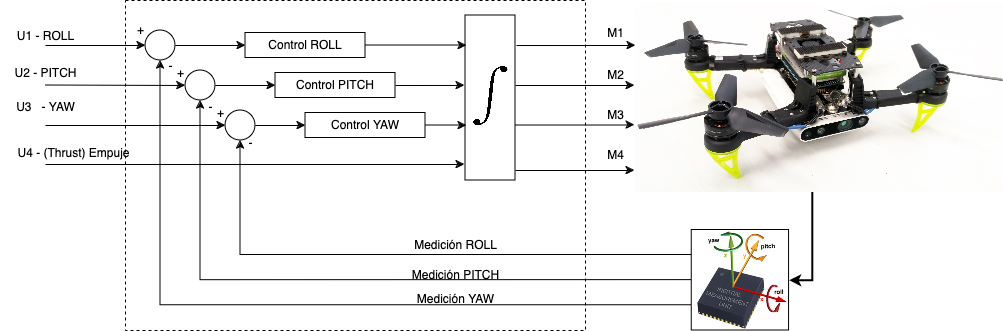
\includegraphics[width=14cm]{drone_control}
  \end{figure}
\end{frame}

%\begin{frame}{Control VANT}
%  \begin{algorithm}[H]
%    \KwData{this text}
%    \KwResult{how to write algorithm with \LaTeX2e }
%    initialization\;
%    \While{not at end of this document}{
%      read current\;
%      \eIf{understand}{
%        go to next section\;
%        current section becomes this one\;
%      }{
%        go back to the beginning of current section\;
%      }
%    }
%    \caption{How to write algorithms}
%  \end{algorithm}
%\end{frame}

\subsubsection{Localización y mapeo simultáneos}

\begin{frame}{Localización (Odometría)}
  
  \begin{minipage}{0.47\textwidth}
    
    \small Un VANT de cuatro rotores cuenta con seis grados de libertar (tres coordenadas lineales x,y,z, tres coordenadas angulares) y cuatro entradas $(u_1,u_2,u_3,u_4)$ o variables de control.\\
    
    Estados del VANT \\
    $(x,y,z,\phi,\theta,\Psi,\dot{x},\dot{y},\dot{z},\dot{\phi},\dot{\theta},\dot{\Psi})^\mathrm{T}$

    \bigskip % Vertical whitespace
    
    Donde:
    \begin{itemize}
    \item $\xi = (x,y,z)^\mathrm{T}$ representan la posición linear
    \item $\eta = (\phi,\theta,\Psi)^\mathrm{T}$ ángulos de euler: roll, pitch, yaw
    \item $(\dot{x},\dot{y},\dot{z},\dot{\phi},\dot{\theta},\dot{\Psi})^\mathrm{T}$ velocidades lineares y angulares
    \end{itemize}
  \end{minipage}
  \hspace{0.2cm}
  \begin{minipage}{0.5\textwidth}
    \centering
    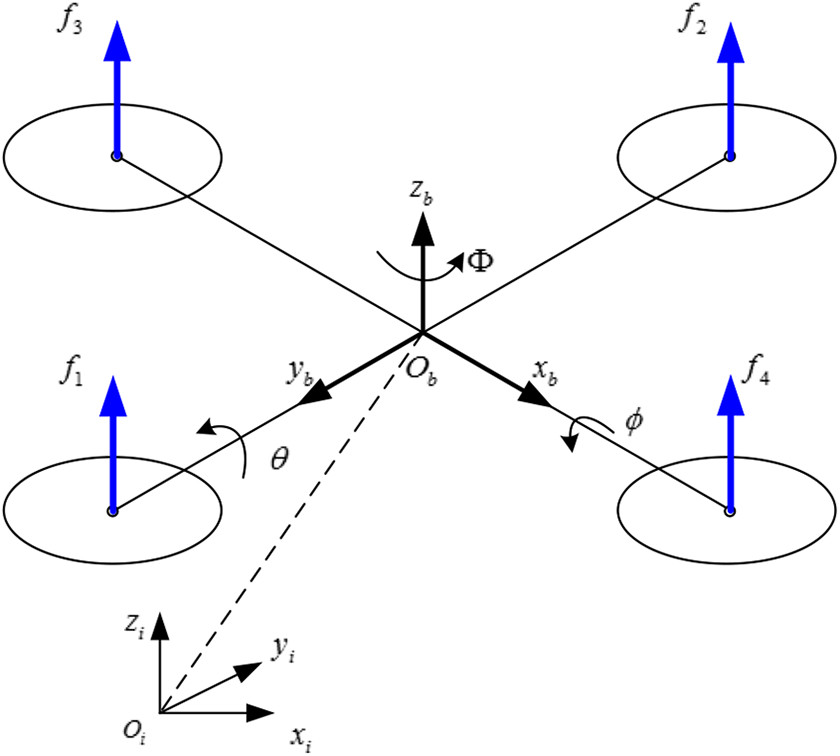
\includegraphics[width=4cm]{uav_model.jpeg}
    \bigskip % Vertical whitespace
  \end{minipage}
\end{frame}

%\begin{frame}
%  \begin{algorithm}[H]
%    \KwData{this text}
%    \KwResult{how to write algorithm with \LaTeX2e }
%    initialization\;
%    \While{not at end of this document}{
%      read current\;
%      \eIf{understand}{
%        go to next section\;
%        current section becomes this one\;
%      }{
%        go back to the beginning of current section\;
%      }
%    }
%    \caption{How to write algorithms}
%  \end{algorithm}
%\end{frame}

\subsubsection{Generación de trayectoria}
\begin{frame}{Generación de trayectoria}
  \begin{minipage}{0.47\textwidth}

    El uso de heuristicas para encontrar soluciones óptimas, proporciona resultados computacionales eficientes. \footnote{A Survey of Trajectory Planning Techniques for Autonomous Systems [\cite{Mir2022}]} 
    \bigskip % Vertical whitespace
    \begin{itemize}
    \item Planificador de trayectoria global
      \begin{itemize}
      \item Búsqueda por grafos
      \end{itemize}
      \bigskip % Vertical whitespace
    \item Planificador de trayectoria local
      \begin{itemize}
      \item Campos de potencial artifical
      \item Algoritmos Bug
      \end{itemize}
    \end{itemize}
    \bigskip % Vertical whitespace
  \end{minipage}
  \hspace{0.2cm}
  \begin{minipage}{0.5\textwidth}
    \centering
    \animategraphics[loop,width=7cm]{10}{video-}{0}{46}
    \rule{0in}{1.2em}$^\dag$\scriptsize Aerial Navigation Development Environment.\\
    \tiny \url{https://www.youtube.com/watch?v=YrtLbCC49kg} 
  \end{minipage}
  
\end{frame}


\begin{frame}{Algoritmo A*}
  \tiny
  \begin{algorithm}[H]
    %\caption{Algoritmo A*}
    \KwData{Inicio, Meta}
    \KwResult{Camino óptimo de Inicio a Meta}
    \BlankLine
    CerrarLista $\gets$ \{\}\;
    AbiertoLista $\gets$ \{\}\;
    \SetKwFunction{Initialize}{Inicializar}
    \SetKwFunction{ExtractMin}{Extraer-Min}
    \SetKwFunction{Insert}{Insertar}
    \SetKwFunction{CostG}{Costo-G}
    \SetKwFunction{CostEdge}{Costo-Arista}
    \SetKwFunction{Heuristic}{Heurística}
    \SetKwFunction{BuildPath}{Construir-Camino}
    \SetKwFunction{UpdateG}{Actualizar-G}
    \SetKwFunction{UpdateParent}{Actualizar-Padre}

    AbiertoLista $\gets$ Inicio \;
    \While{\textup{\textbf{no está vacía}}(AbiertoLista)}{
      Actual $\gets$ \ExtractMin{AbiertoLista} \;
      \Insert{CerrarLista, Actual} \;
    
      \If{Actual $=$ Meta}{
        \Return \BuildPath{Inicio, Meta} \;
      }

      \ForEach{vecino $v$ de Actual}{
        \If{$v$ está en CerrarLista}{
          \textbf{continuar} \;
        }
        
        $g \gets$ \CostG{Inicio, Actual} $+$ \CostEdge{Actual, $v$} \;
        $h \gets$ \Heuristic{$v$, Meta} \;
        $f \gets g + h$ \;
        
        \If{$v$ \textup{\textbf{no está en}} AbiertoLista}{
          \Insert{AbiertoLista, $v$} \;
        }\ElseIf{$g \geq$ \CostG{Inicio, $v$}}{
          \textbf{continuar} \;
        }
        
        \UpdateG{Inicio, $v$, $g$} \;
        \UpdateParent{$v$, Actual} \;
      }
    }
    
    \Return \textup{\textbf{Sin-Solución}} \;
  \end{algorithm}
\end{frame}

\begin{frame}{Campo de potencial artificial}
  \tiny
  \begin{algorithm}[H]
        
    %\KwData{Posición del robot $robotPos$, Posición objetivo $objetivoPos$, Lista de obstáculos $obstaculos$}
    %\KwResult{Mensaje indicando si se alcanzó el objetivo}
    
    %\SetKwFunction{DistanciaEntre}{distancia\_entre}
    %\SetKwFunction{Normalizar}{normalizar}
    
    %\SetKwInOut{Parameter}{Parámetros}
    %\Parameter{$k\_atractivo$: constante de atracción, $k\_repulsivo$: constante de repulsión, $r\_repulsivo$: radio de influencia repulsiva, $paso\_t$: tamaño del paso de tiempo}
    
    %\BlankLine
    %Inicializar velocidad del robot: $Velocidad \gets [0, 0]$\;

    El VANT sigue la trayectoria generado por el planificador global\;

    \eIf{Objetivo alcanzado}{
      Parar navegación\;
    }{
      \eIf{Se detecta obstáculo}{
        Comportamiento APF\;
        Cálculos APF\;
        Girar respecto al ángulo calculado para encontrar la siguiente posición segura a moverse\;
        \If{Objetivo alcanzado}{
          Parar navegación\;
        }
        \If{Se detecta obstáculo}{
          Repetir comportamiento APF\;
        }
      }{
        Seguir navegando hasta encontrar el objetivo o encontrar un obstáculo\;
      }
      
    }
        
  \end{algorithm}
\end{frame}

\section{Coordinación multi-VANT}
\begin{frame}{Coordinación multi-VANT}
  \begin{minipage}{0.47\textwidth}
    \begin{itemize}
    %\item Exploración con algoritmos de baja complejidad computacional.
    \item Centralizada: Una entidad planea para todos los robots. (El problema crece conforme aumentan los robots)
    \item Decentralizada: Cada robot es completamente independiente y planea sus propios trayectos
    \end{itemize}
  \end{minipage}
  \hspace{0.2cm}
  \begin{minipage}{0.5\textwidth}
    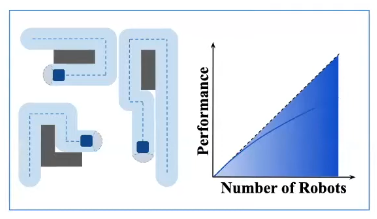
\includegraphics[width=0.8\textwidth]{coordination}$^\dag$\\
      \rule{0in}{1.2em}$^\dag$\scriptsize \cite{amanda}
  \end{minipage}
\end{frame}


\begin{frame}{Problema de asignación}
  \begin{minipage}{0.48\textwidth}
    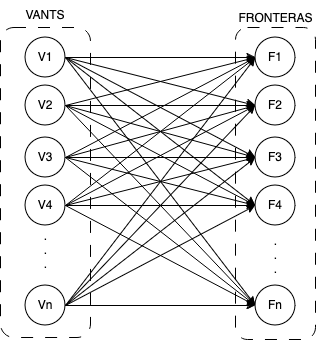
\includegraphics[width=0.8\textwidth]{asignacion}%$^\dag$\\
    %\rule{0in}{1.2em}$^\dag$\scriptsize \cite{amanda}
  \end{minipage}
  %\hspace{0.1cm}
  \begin{minipage}{0.51\textwidth}

    El problema del emparejamiento ponderado en un grafo bipartito, también conocido como problema de asignación.
    
    \begin{itemize}
    \item un conjunto $N$ de $n$ agentes;
    \item un conjunto $X$ de $n$ tareas;
    \item un conjunto $M \subseteq N \times X$ de posibles pares;
    \item una función $v : M \mapsto \mathbb{R}$ que calcula cada par de asignación;
    \end{itemize}
    \begin{block}{Corolario}
      El problema de asignación puede ser resuelto en un tiempo polinomial. $O(n^{3})$ \footnote{\cite{multi-book}}
    \end{block}
  \end{minipage}
\end{frame}

\begin{frame}{Algoritmos para el problema de asignación \footnote{The assignment problem revisited, \cite{Alfaro2021}}}

  \begin{itemize}
  \item 1955 - Kuhn propuso el primer algoritmo para resolver el problema en tiempo polinomial \textbf{$O(mn+n^{2}\log(n))$}.
  \item 1992 - Algoritmo Bertsekas $\epsilon$ - scaling auction \textbf{$O(nm\log(nW))$} (paralelizable solo para instancias balanceadas).
  \item 1995 - Algoritmo Goldberg \& Kennedy \textbf{$O(m\sqrt{s}\log(sW)$}. 
  \item El algoritmo $\epsilon$ - scaling auction y el algoritmo Goldberg \& Kennedy tienen un mismo rendimiento para instancias pequeñas. 
  \item Para instancias mayores el algoritmo $\epsilon$ - scaling auction tiene un mayor desempeño que los otros algoritmos.
  \end{itemize}
\end{frame}


\section{Simulación}
\begin{frame}{Simulación}
  El simulador dinámico \cite{RACER2022} \footnote{Rapid Collaborative Exploration With a Decentralized Multi-UAV System} utiliza la odometría de referencia de los VANTS, suponiendo que cada agente está equipado con una cámara de profundidad que mira hacia adelante cuya resolución es 640x480px y un campo de visión de 80°x60°. Las imágenes de profundidad se generan utilizando el proceso presentado en \cite{OMNI2022} \footnote{Omni-Swarm: A Decentralized Omnidirectional Visual–Inertial–UWB State Estimation System for Aerial Swarms} con un rango máximo de detección de 4.5 m.
  \bigskip % Vertical whitespace
  \begin{itemize}
  \item En tiempo necesario para completar la exploración del ambiente dado y la velocidad promedio de los VANTS durante cada experimento.
  \item Tasas de exploración para diferentes cantidades de VANTS en diversos ambientes.
  \end{itemize}
\end{frame}

%\begin{frame}{Simulación}
%  \textbf{Robot Operating System (ROS)}\\
%  \bigskip % Vertical whitespace
%  \begin{itemize}
%  \item Provee un conjunto de herramientas usadas por un robot (Sensores, actuadores, implementación diversos algoritmos)
%  \item Framework de comunicación que permite interconectar las diferentes piezas del cerebro para hablar con otras lecturas de sensores.
%  \end{itemize}
%  \bigskip % Vertical whitespace
%  En resumen ROS ayuda en descomponer software complejos en pequeñas piezas más manejables. 
%\end{frame}

\begin{frame}{ROS Master}
  \begin{figure}
    \centering
    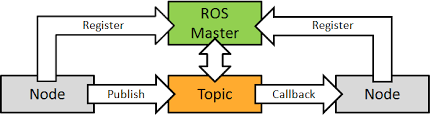
\includegraphics[width=0.5\textwidth]{ros_master}
  \end{figure}
  
  \begin{itemize}
    \item Es un servidor que provee información de conexión (dirección, notificaciones) hacia los nodos del sistema.
    \item Los mensajes son transmitidos entre los nodos vía peer-to-peer.
    \item Los nodos deben conocer la dirección del nodo maestro antes de iniciar.
    \item Los nodos son programas individuales y se organizan en paquetes.
    \item La comunicación entre nodos es mediante tópicos y es de tipo unidireccional.
  \end{itemize}
\end{frame}

\begin{frame}{Visualización interacción nodos en ROS}
  \begin{figure}
    \centering
    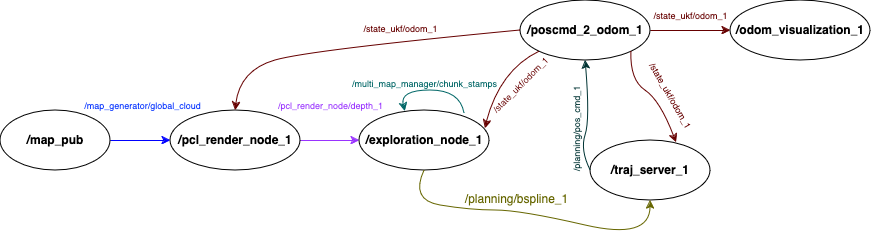
\includegraphics[width=1\textwidth]{ros_nodes}
  \end{figure}
\end{frame}

\begin{frame}{Avance Simulación}
  \begin{figure}
    \centering
    \animategraphics[loop,width=8cm]{10}{path/frame_}{000}{220}
  \end{figure}
\end{frame}

%\begin{frame}{Representación del Medio Ambiente - ¿Dónde estoy?}
%  \bigskip % Vertical whitespace
%  \centering
%  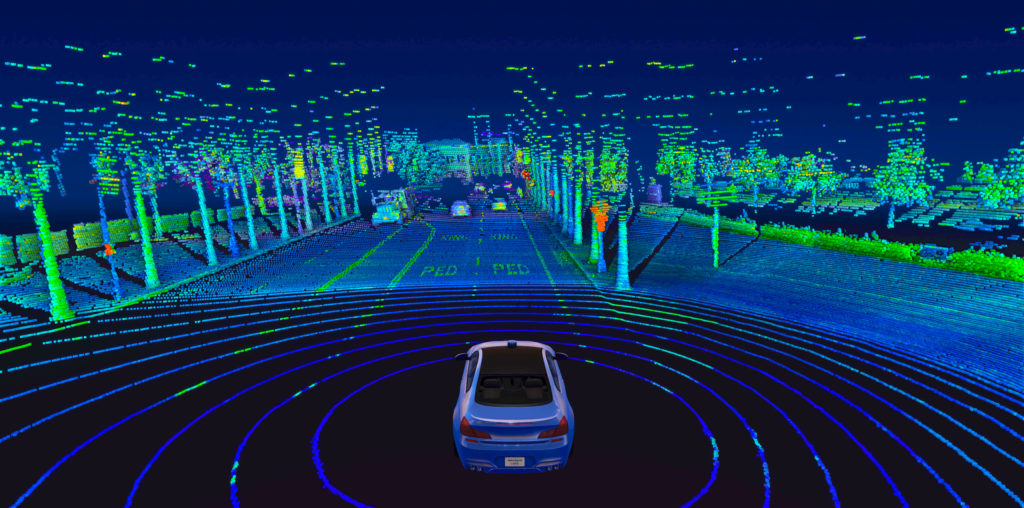
\includegraphics[width=0.45\textwidth,height=0.35\textheight]{map3d.jpg}
%  \hfil
%  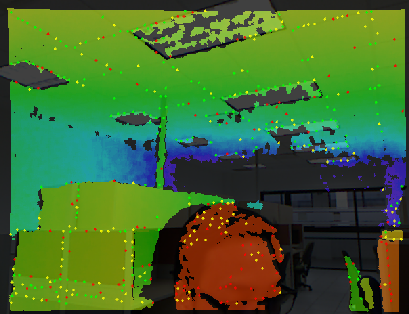
\includegraphics[width=0.45\textwidth,height=0.35\textheight]{rgbd}
%  \vspace{2pt}\\
%  \bigskip % Vertical whitespace
%  Es la construcción de un mapa del entorno, realizada por un robot, utilizando información espacial obtenida durante el paso del tiempo. [\citeauthor{Wallgrn2010} 2010]\\
%  \bigskip % Vertical whitespace
%  Fuentes de información:
%  \begin{itemize}
%  \item Escáners láser tipo LIDAR.
%  \item Cámaras RGB-D.
%  \end{itemize}  

%  \bigskip % Vertical whitespace
  
%  \tiny La precisión del mapa debe corresponder con la precisión con la cual el robot necesita cumplir sus tareas.
  
  %
\includegraphics[width=0.45\textwidth,height=0.35\textheight]{DJI_B5}$^\dag$ 
  %\hfil
  %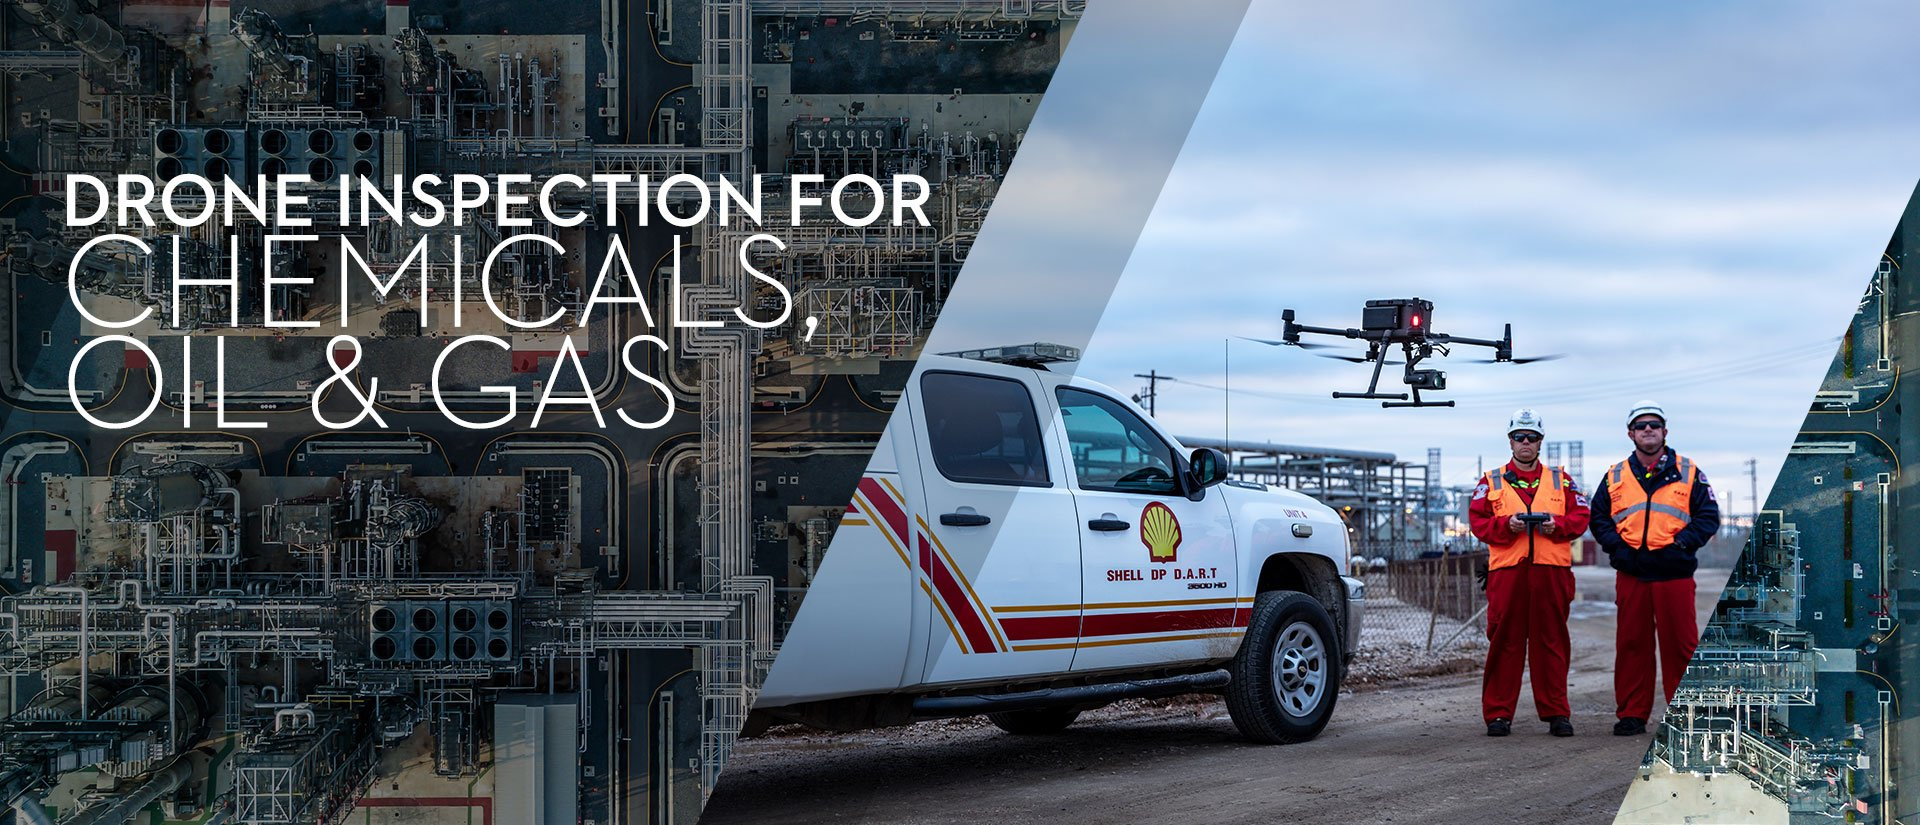
\includegraphics[width=0.45\textwidth,height=0.35\textheight]{DJI_B4}$^\dag$\\
  %\rule{0in}{1.2em}$^\dag$ \small Inspecciones con VANT basadas en los mejores casos de uso\\
  %\tiny \url{https://enterprise-insights.dji.com/blog/complete-guide-to-drone-inspections}
%\end{frame}

%\begin{frame}{Representación del Medio Ambiente - ¿Dónde estoy?}
%  \centering
%  \begin{figure}[h]
%    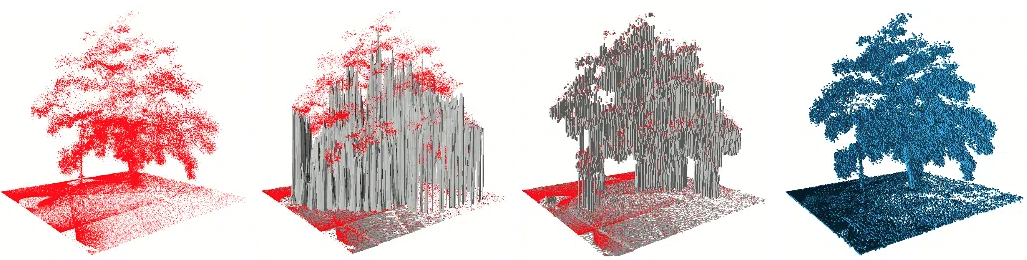
\includegraphics[width=0.8\textwidth,height=0.35\textheight]{img4}%\footnotemark 
%    {\tiny \caption{Nube de puntos, Mapa de elevación, Superficies multi-nivel, Octomap}}
%  \end{figure}
  
%  \addvspace{\medskipamount}
%  \noindent
%  \begin{tabularx}{\linewidth}{ @{} X X @{} }
    
%    \begin{figure}[h]
%      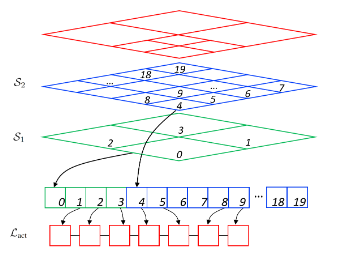
\includegraphics[width=0.2\textwidth,height=0.3\textheight]{hgrid}
%      {\tiny \caption{HGrid}}
%    \end{figure}
%    &
%    \begin{figure}[h]
%      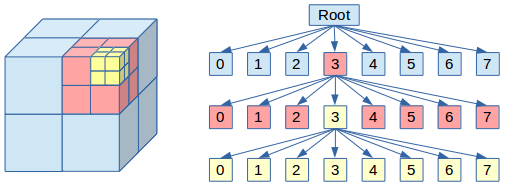
\includegraphics[width=0.4\textwidth,height=0.3\textheight]{octree}
%      {\tiny \caption{Octree}}
%    \end{figure}
    
%  \end{tabularx}

  %\footnotetext{\tiny OctoMap: An Efficient Probabilistic 3D Mapping Framework Based on Octrees [\cite{hornung13auro}]}
  
%\end{frame}

%\begin{frame}{Representación del Medio Ambiente - ¿Dónde estoy?}

%  \begin{itemize}
%  \item Hierarchical Grid (HGrid)
%    \begin{itemize}
%    \item Funciona bien para consultas de vecinos cercanos y búsquedas en un espacio tridimensional.
%    \item Similar a la descomposición de un octree, pero su implementación con arrays le permite una complejidad $O(1)$ para consultas.
%    \item Puede requerir más memoria dependiendo de la resolución de la cuadrícula y la complejidad de la función hash.
%    \end{itemize}
%  \item Octomap (Octree).
%    \begin{itemize}
%    \item Tiende a ser más compacto en términos de almacenamiento de datos que algunas cuadrículas hash.
%    \item Utiliza una estructura de árbol octree para representar la ocupación del espacio de manera eficiente.
%    \item La actualización dinámica puede ser más desafiante y requerir técnicas adicionales.
%    \end{itemize}
%  \end{itemize}  
%\end{frame}

%\begin{frame}{Toma de decisiones - ¿A dónde voy?}
  %\centering
%  \begin{figure}[h]
%    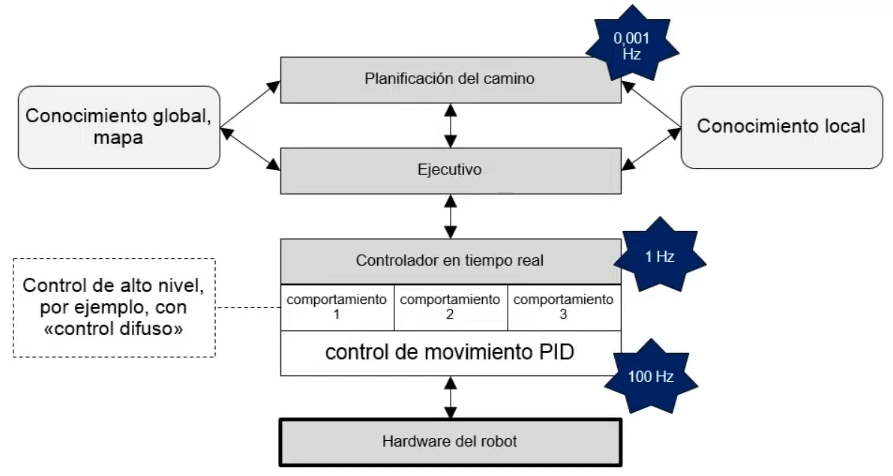
\includegraphics[width=0.65\textwidth]{arq_basica}
%    \caption{Arquitectura básica de un robot móvil}
%  \end{figure}
%  \bigskip % Vertical whitespace
%  \tiny Un sistema de control para un robot móvil autónomo opera en un entorno donde las condiciones están cambiando rápidamente. (considerando el problema de control instantáneo en una formulación clásica de teoría de control) \\\footnote{{\tiny robust layered control system for a mobile robot [\cite{brooks_robot}]}}
  
%\end{frame}

%\begin{frame}{Arquitectura híbrida}
%  \begin{minipage}{0.47\textwidth}
    
%    \small El robot puede reaccionar de manera rápida a estímulos del entorno, al mismo tiempo que tiene la capacidad de planificar y tomar decisiones de alto nivel.
    
%    \begin{itemize}
%    \item Adaptable al lidiar con situaciones predecibles como imprevistas.
%    \item Permite una respuesta rápida a estímulos del entorno.
%    \item Optmiza el rendimiento del robot al gestionar las tareas simples y repetitivas, liberando recursos para tareas deliberativas más complejas.
%    \item Es escalable.
%    \end{itemize}
%  \end{minipage}
%  \hspace{0.2cm}
%  \begin{minipage}{0.5\textwidth}
%    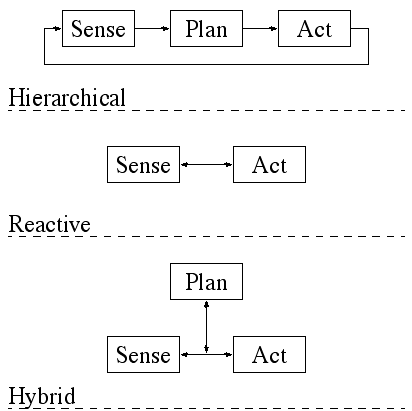
\includegraphics[width=0.8\textwidth]{architecture.png}$^\dag$\\
%    \rule{0in}{1.2em}$^\dag$\scriptsize Ciclo Sense-Plan-Act \\
%    \tiny \cite{murphy2000} %https://cs.brown.edu/people/tdean/courses/cs148/02/architectures.html#Murphy
%  \end{minipage}
%\end{frame}

%\begin{frame}{Planificación de trayectoria - ¿Cómo llego hasta ahí?}
%  \bigskip % Vertical whitespace
%  \centering
%  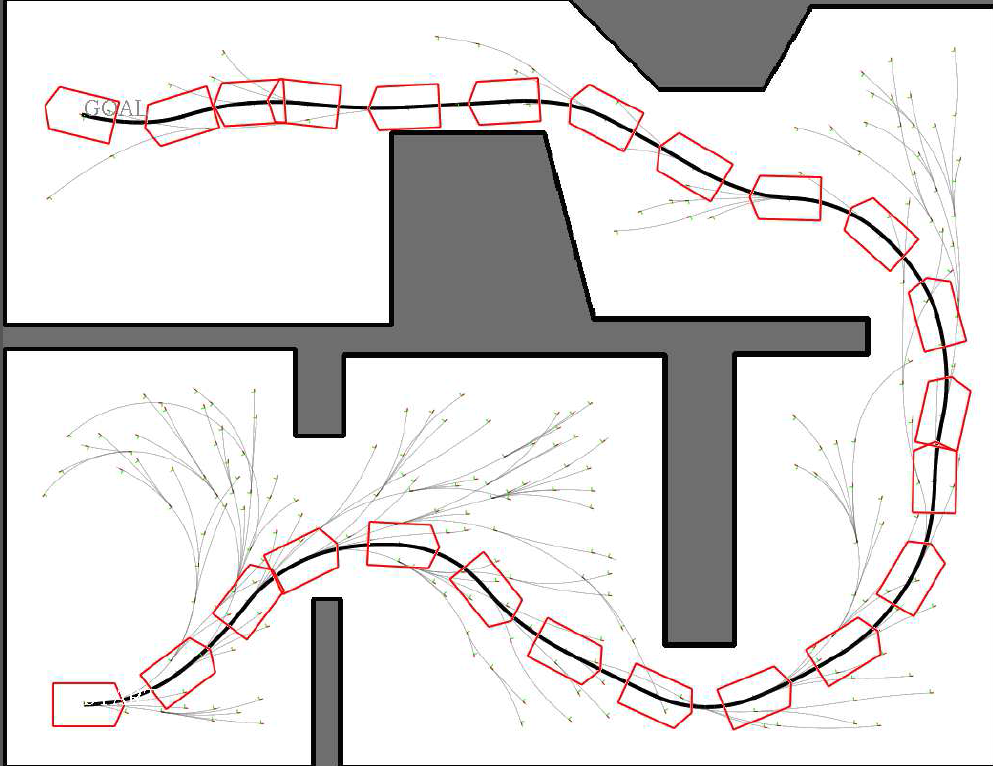
\includegraphics[width=0.45\textwidth,height=0.30\textheight]{rrt}
%  \hfil
%  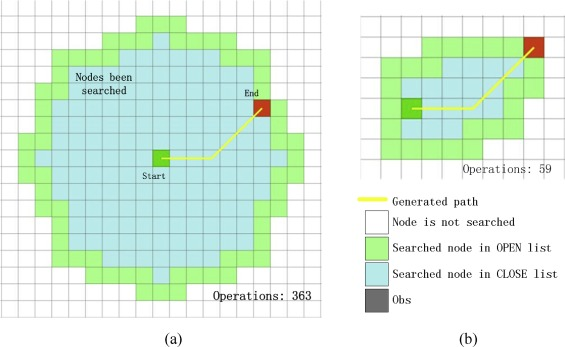
\includegraphics[width=0.45\textwidth,height=0.30\textheight]{astar.jpg}
%  \vspace{0.5pt}\\
  %\bigskip % Vertical whitespace
  %Indica a un robot como moverse de un punto a otro en su entorno. Implica la generación de trayectorias y movimientos que permiten a los robots cumplir sus tareas o alcanzar sus objetivos mientras evitan obstáculos \footnotemark.}\\
%  \bigskip % Vertical whitespace
%  \addvspace{\medskipamount}
%  \noindent
%  \begin{tabularx}{\linewidth}{ @{} X X @{} }
%    Por Grafos \footnotemark
    
%    \begin{itemize}
%    \item Grafos de visibilidad. 
%    \item Diagramas de Voronoi.
%    \item Descomposición por celdas.
%    \item Arboles de exploración rápida (RRT).
%    \item Consulta múltiple (PRM)
%    \end{itemize} &

%    Algoritmos
    
%    \begin{itemize}
%    \item BFS (a) , DFS
%    \item A* (b), D*
%    \item Dijkstra
%    \end{itemize}
%  \end{tabularx}
%  \footnotetext{{\tiny Different Cell Decomposition Path Planning Methods for Unmanned Air Vehicles A Review [\cite{Debnath2020}]}}
%\end{frame}

\section{Conclusiones}
\begin{frame}{Discusión}
  
  \begin{block}{Hipótesis}
    Una estrategia que coordine y asigne tareas de exploración para múltiples VANTS, en combinación con una arquitectura de software (que resuelva los problemas de localización, manejo de mapas y planificación de rutas) mejorará el desempeño en tareas de exploración con múltiples VANTS en entornos desconocidos.
  \end{block}

  \begin{itemize}
    \item Elección de un simulador ligero compatible con ROS.
    \item Resolver el problema de autónomia para cada agente nos aproxima a validar la hipótesis planteada.
    \item Dividir el problema en agentes individuales nos ayuda a su comprensión, y hace que el mecanismo de coordinación tome un papel importante en compañia de una función que modele las fronteras a explorar. 
  \end{itemize}
\end{frame}

\begin{frame}{Discusión}
  \scriptsize
  \begin{block}{Preguntas investigación}
    \begin{itemize}
    \item ¿Qué mecanismos de coordinación existen dentro de la literatura que podrían ayudar en resolver el problema de exploración multi-VANT?\\
    \item ¿Qué características de la dinámica del robot se deben considerar en el simulador, para que los resultados se aproximen a los del mundo real?\\
    \item ¿Es posible que el uso de una estructura de datos como octree para representar la ocupación de un volumen, sea más eficiente que una representación usando una matriz cúbica?\\
    \end{itemize}
  \end{block}
  \begin{itemize}
  \item La comparación de mecanismos de coordinación es interesante, muchos trabajos en multi-robots siguen usando un enfoque de coordinación bajeo el uso del algoritmo húngaro.
  \item El simulador dinámico \cite{RACER2022} \footnote{\tiny Rapid Collaborative Exploration With a Decentralized Multi-UAV System} utiliza la odometría de referencia de los VANTS, suponiendo que cada agente está equipado con una cámara de profundidad que mira hacia adelante cuya resolución es 640x480px y un campo de visión de 80°x60°.
  \item Las imágenes de profundidad se generan utilizando el proceso presentado en \cite{OMNI2022} \footnote{\tiny Omni-Swarm: A Decentralized Omnidirectional Visual–Inertial–UWB State Estimation System for Aerial Swarms} con un rango máximo de detección de 4.5 m.
  \end{itemize}
\end{frame}

\begin{frame}[allowframebreaks,noframenumbering]{Bibliografía}
  \tiny
  \bibliographystyle{abbrvnat}
  \bibliography{test}
\end{frame}

\end{document} 
